\documentclass[11pt]{exam}
\usepackage{../commonheader}
\usepackage{graphicx}

\title{Homogeneous Systems, Rank, Matrix Arithmetic}
\date{Week 2, Session 1}

\begin{document}
\maketitle

\section{Homogeneous Systems}

    Recall that homogeneous systems have the form:
    $$a_{11}x_1 + a_{12}x_2 + \dots + a_{1n}x_n = 0$$
    $$a_{21}x_1 + a_{22}x_2 + \dots + a_{2n}x_n = 0$$
    $$\vdots$$
    $$a_{m1}x_1 + a_{m2}x_2 + \dots + a_{mn}x_n = 0$$

    Equivalently:
    $$\begin{amatrix}{4}
        a_{11} & a_{12} & \dots & a_{1n} & 0 \\
        a_{21} & a_{22} & \dots & a_{2n} & 0 \\
        \vdots & \vdots & \vdots & \vdots & \vdots \\
        a_{m1} & a_{m2} & \dots & a_{mn} & 0 \\
    \end{amatrix}$$
    
    \vspace{20px}
    \subsection{Trivial Solution of Homogeneous Systems}
        \begin{questions}
            \item Fill in the blank: Homogeneous systems always have at least \rule{5mm}{0.15mm} solution(s).
            \item Fill in the blank: If a homogeneous system has a solution in which not all of the $x_1 \dots x_n$ are equal to zero,
            this solution is called a \rule{5mm}{0.15mm} solution.
            \item Consider a three-variable homogeneous system. For its trivial solution, what are the values of $x, y, z$?
        \end{questions}

    \vspace{20px}
    \subsection{Basic Solutions of Homogeneous Systems}
        \begin{questions}
            \item Consider a homogeneous system with the following solution:
            $$\begin{bmatrix} x \\ y \\ z \end{bmatrix}
            = \begin{bmatrix} 0 \\ 0 \\ 0 \end{bmatrix}
            + s \begin{bmatrix} 2 \\ 1 \\ 2 \end{bmatrix}
            + t \begin{bmatrix} 0 \\ 1 \\ 1 \end{bmatrix}$$
            What are the basic solution(s) of this system?

            \item Find the basic solution(s) (if any) of the following homogeneous system: \\
            $\begin{amatrix}{2}
                1 & 2 & 0 \\
                4 & 8 & 0
            \end{amatrix}$

            \item Find the basic solution(s) (if any) of the following homogeneous system: \\
            $\begin{amatrix}{3}
                1 & 1 & 6 & 0 \\
                1 & 3 & 14 & 0 \\
                2 & 2 & 12 & 0
            \end{amatrix}$
        \end{questions}

        \vspace{20px}
        We say that the set of solutions of a homogeneous system is a \textit{linear combination} of the basic solutions.

        For example, if a homogeneous system has two basic solutions $X_1$ and $X_2$, the set of solutions of the system can
        be expressed as $X = sX_1 + tX_2$, where $s,t$ are real numbers. In essence, $X$ is a "list" of any points that can be
        "reached" by combining some "amount" of $X_1$ and $X_2$.

        To try to build some intuition, consider the following graphical example.
        Suppose the red/blue arrows are two vectors which are basic solutions of a system.
        \begin{center}
            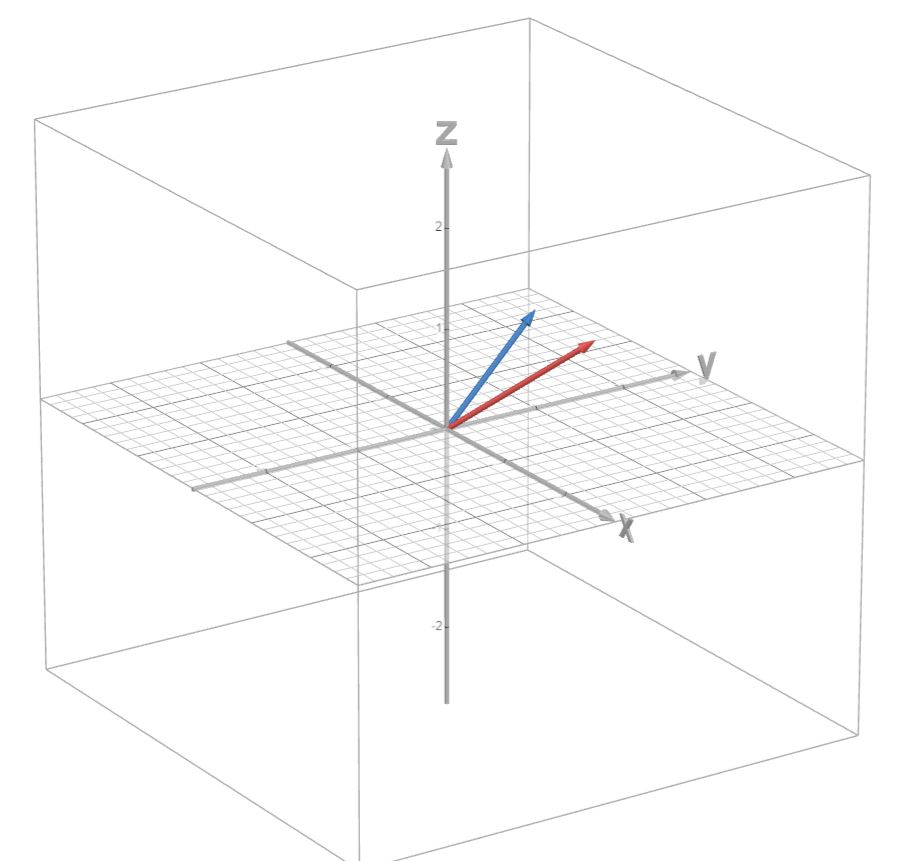
\includegraphics[width=0.5\textwidth]{vectors.JPG}
        \end{center}

        \pagebreak
        These two vectors define a plane that both vectors lie within; any point in this plane can be reached by combining these two vectors
        in some amounts!
        \begin{center}
            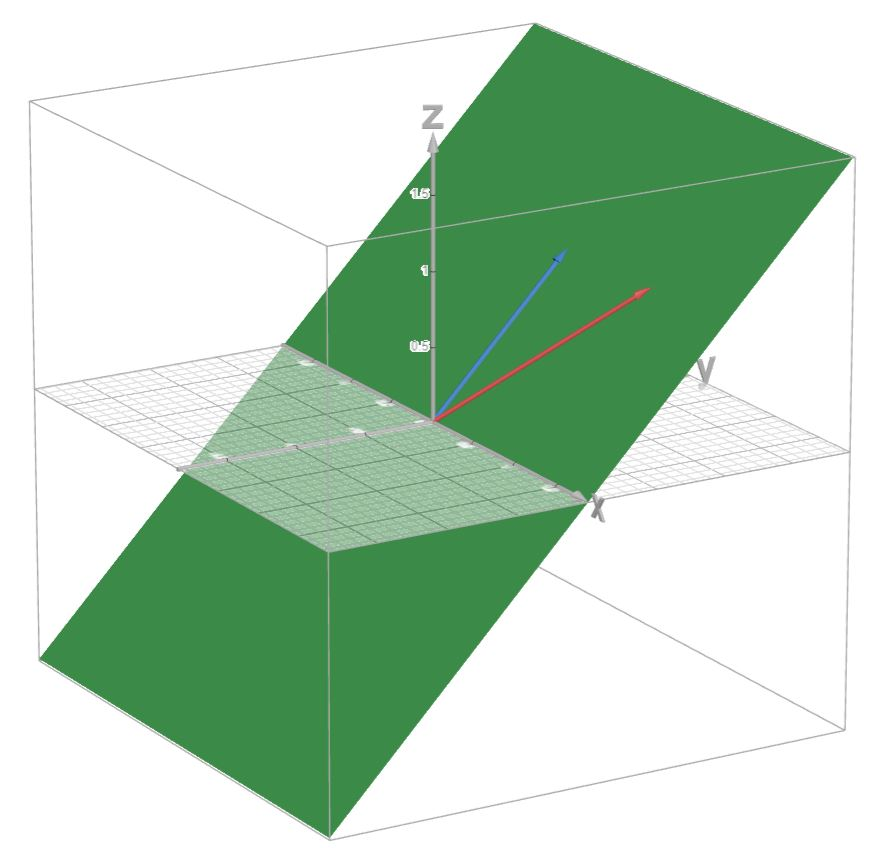
\includegraphics[width=0.5\textwidth]{plane.JPG}
        \end{center}
    
    \vspace{20px}
    \subsection{Matrix Sizes and Nontrivial Solutions}
        When the \textit{coefficient matrix} of the homogeneous system (that is, the matrix without the augmented row) has fewer rows
        than columns, it turns out that the system will \textit{always} have a nontrivial solution!

        Reason: Remember that each row is a separate equation, and each column is a variable. When we have fewer equations than variables,
        it's impossible to construct equations such that all variables have a single unique value, so we will have infinite solutions. Since
        we have infinite solutions, there must be at least one parameter.

        We normally say a matrix has $m$ rows and $n$ columns. With that in mind, let's try to answer the following conceptual questions:

        \begin{questions}
            \item When $m = n$ for a homogeneous system, will we always, never, or sometimes have a nontrivial solution?
            \item When $m > n$ for a homogeneous system, will we always, never, or sometimes have a nontrivial solution?
        \end{questions}


\pagebreak
\section{Rank}
    The \textit{rank} of a matrix is the number of pivot columns in the row-echelon or reduced row-echelon forms of the matrix.
    For a matrix $A$, we can write this as $\text{Rank}(A)$.

    For an $m \times n$ coefficient matrix with rank $r$, the solution to the system will have $n - r$ parameters/free variables/basic solutions.

    \begin{questions}
        \item Consider the following $3 \times 3$ homogeneous system, already reduced to RREF:
        $$\begin{amatrix}{3}
            1 & 0 & 1 & 0 \\
            0 & 1 & 2 & 0 \\
            0 & 0 & 0 & 0
        \end{amatrix}$$
        \begin{enumerate}
            \item What is the rank of this matrix?
            \item How many parameters will the solution to this system have?
        \end{enumerate}
    \end{questions}

    \vspace{20px}
    \subsection{Rank and Consistent Systems}
    Now, let's consider how we can use rank for non-homogeneous, consistent systems. Note that non-homogeneous systems \textit{can be} inconsistent;
    if that's the case, none of this discussion applies.

    \begin{enumerate}
        \item When the rank $r$ of a consistent system is less than the number of variables $n$, the system will have at least one parameter.
        Thus it will have infinite solutions.
        \item When the rank $r$ of a system is equal to the number of variables $n$, the system doesn't have any parameters.
        Thus, there is either exactly one or no solutions. Since we presupposed the system to be consistent, it has exactly one solution.
    \end{enumerate}

    Again, the rank of a system does not determine the consistency or inconsistency of a system in any way!

    \begin{questions}
        \item Use the concepts of rank and consistency to classify the number of solutions and parameters (if any) of the following
        non-homogeneous systems:
        \begin{enumerate}
            \item $\begin{amatrix}{3}
                1 & 0 & 0 & 1 \\
                0 & 1 & 0 & 2 \\
                0 & 0 & 1 & 3 \\
            \end{amatrix}$
            \item $\begin{amatrix}{3}
                1 & 0 & 2 & 1 \\
                0 & 1 & 3 & 1 \\
                0 & 0 & 0 & 0 \\
            \end{amatrix}$
            \item $\begin{amatrix}{3}
                1 & 0 & 5 & 1 \\
                0 & 1 & 5 & 1 \\
                0 & 0 & 0 & 1 \\
            \end{amatrix}$
        \end{enumerate}     
    \end{questions}

\pagebreak
\section{Matrix Arithmetic}

    \vspace{20px}
    \subsection{Introduction}
        \begin{questions}
            \item A square matrix has \textbf{3} rows. How many columns does it have?
            \item A $3 \times 3$ zero matrix has \textbf{3} rows and \textbf{3} columns. What is the value of the top-leftmost entry?
            \item Two $2 \times 2$ matrices, $A$ and $B$ have the same set of entries, but listed in different orders in the matrix. Does $A = B$?
        \end{questions}

    \vspace{20px}
    \subsection{Matrix Addition}
        \begin{questions}
            \item Perform the following matrix additions:
            \begin{enumerate}
                \item $\begin{bmatrix} 1 & 1 \\ 2 & 2 \end{bmatrix} + \begin{bmatrix} 2 & 2 \\ 3 & 4 \end{bmatrix}$
                \item $\begin{bmatrix} 0 & 1 \end{bmatrix} + \begin{bmatrix} 1 & 2 \end{bmatrix}$
                \item $\begin{bmatrix} 1 & 1 \\ 2 & 2 \end{bmatrix} + \begin{bmatrix} 2 & 2 \end{bmatrix}$
            \end{enumerate}
        \end{questions}

    \vspace{20px}
    \subsection{Scalar Multiplication of Matrices}
        \begin{questions}
            \item Perform the following scalar matrix multiplications:
            \begin{enumerate}
                \item 3 $\times \begin{bmatrix} 1 & 1 \\ 2 & 2 \end{bmatrix}$
                \item $\frac{3}{2} \times \begin{bmatrix} 1 & 5 \end{bmatrix}$
                \item $0 \times \begin{bmatrix} 1 & 1 \\ 2 & 2 \end{bmatrix}$
            \end{enumerate}
        \end{questions}

    \pagebreak
    \section{Closing}
    Let's wrap today's session up with some summarizing questions!
    \begin{questions}
        \item Suppose a homogeneous system is found to have two basic solutions. How many free variables does the system have, and how many
        solutions does the system have?
        \item Suppose a $5 \times 3$ homogeneous system has rank 3. How many free variables does the system have, and how many
        solutions does the system have?
        \item Fill in the blank: Rank is the number of \rule{5mm}{0.15mm} columns in a system.

        \item Consider the following system:

        $\begin{amatrix}{3}
            1 & 2 & 3 & 1 \\
            0 & 0 & 0 & 1 \\
            0 & 0 & 0 & 0
        \end{amatrix}$ \\

        What is the rank of the system? How many solutions does it have?

        \item Find the value of matrix $A$:
        
        $A = 2 \begin{bmatrix} 3 & 2 \\ 2 & 4 \end{bmatrix} - 3 \begin{bmatrix} 1 & 1 \\ 0 & 1 \end{bmatrix}$
    \end{questions}

\end{document}